\chapter {Implementacja}
\label{cha:implementacja}
Poniższy rozdział zawiera przegląd ciekawszych aspektów implementacyjnych projektu.
Na wstępie omówiono użyte technologie oraz narzędzia wraz z uzasadnieniem wyboru. Następnie przedstawiono dokładny model aplikacji z uwzględnieniem wybranych metod implementacyjnych. 
W rozdziale tym przedstawiono także problemy, z którymi zetknęli się autorzy podczas realizacji projektu oraz sposoby ich rozwiązania.
\section {Wybrane technologie i narzędzia}
Przed przystąpieniem do implementacji końcowej wersji aplikacji powstawały prototypy testujące różne podejścia algorytmiczne opisane w rozdziale \ref{cha:Algorytm} oraz możliwe do wykorzystania narzędzia. W sekcji \textit{Język implementacji} przedstawiono język wybrany do implementacji końcowej wersji programu, natomiast w sekcji \textit{Języki prototypowania} przedstawiono technologie używane do tworzenia prototypów systemu. Następnie pokrótce omówiono narzędzia pracy grupowej wykorzysywane podczas realizacji projektu Sparkle.
\subsection{Język implementacji}
Do implementacji końcowej wersji aplikacji został wybrany język Java.
Język ten został wybrany ze względu na przenośność aplikacji, obiektowość ułatwiającą projektowanie, dostęp do licznych 
bibliotek oraz mechanizmy pozwalające uchronić program przed wyciekami pamięci krytycznymi z punktu widzenia aplikacji czasu rzeczywistego. Innym, rozważanym językiem implementacji był język C++. Przed końcowym wyborem zostały przeprowadzone badania dotyczące wydajności rozważanych języków. Przyniosły one następujące rezultaty:
%http://java.sun.com/docs/performance/ - może z tego uda się coś wyciągnąć o efektywności javy
\begin{itemize}

\end{itemize}

\subsection{Języki prototypowania}
Jednym z powstałych ptotypów był prosty automat komórkowy z regułami opisanymi w paragrafie [WSTAWIC ODNOSNIK DO PARAGRAGU].Do implementacji tego modelu został korzystany język Lisp.
\\\\
[TUTAJ WSTAWIC ZALETY LISPA DO PROTOTYPOWANIA - WYMYSLISZ COS PRAWDA :>?]
\\
Drugim, powstałym podczas badań pierwowzorem był program napisany w języku Java.
Celem tego modelu było przetestowanie języka Java oraz biblioteki Java3D pod kątem możliwości wykorzystania do implementacji symulacji czasu rzeczywistego w oparciu o uproszczony model automatu. 

\subsection {Narzędzia pracy grupowej}
Ze względu na fakt, że omawiana aplikacja powstała jako wynik pracy dwuosobowego zespołu bardzo przydatnym narzędziem okazał się system kontroli wersji. Jako system zarządzania wersjami został wybrany Git.
Git jest darmowym, rozproszonym systemem, opartym na architekturze peer-to-peer. W przeciwieństwie do scentralizowanych odpowiedników (np. SVN) nie posiada jednego, centralnego repozytorium z którym członkowie zespołu synchronizują swoje zmiany ale wiele niezależnych gałęzi, które można synchronizować w różnorodny sposób. Główną zaletą systemu Git, będącą motywacją jego wyboru...

\section {Implementacja modelu aplikacji}
Zgodnie z architekturą aplikacji omówioną w rozdziale \ref{cha:projekt} program został podzielony na 
\begin{itemize}
\item Moduł wizualizacji danych
\item Moduł realizujący logikę aplikacji
\item Moduł kontrolera, odpowiadający za interakcje z użytkownikiem.
\end{itemize}
Poniżej przedstawiono najważniejsze implementacyjne aspekty realizacji poszczególnych modułów.
Opis implementacji wzbogacony został o diagramy klas UML przedstawiające budowę poszczególnych pakietów, zwracające uwagę na powiązania między jednostkami oraz uwypuklające wybrane metody implementacyjne.
\subsection {Moduł wizualizacji}
Wizualizacja symulacji została zaimplementowana z wykorzystaniem Java3D API.
Java3D to interfejs programowy (API) umożliwiający tworzenie trójwymiarowej grafiki. Jest to produkt firmy Sun Microsystems wykorzystujący w swoim działaniu renderery OpenGL i Direct3D w zależności od platformy.
Główną zaletą determinująca wybór bilioteki Java3D jest umożliwienie wykorzystania technologii OpenGL i DirectX poprzez dostarczenie wysokopoziomowych struktur pozwalających zachować pełnię obiektowości języka Java. 
Zastosowana w bibliotece Java3D obiektowość ułatwia zarządzanie elementami sceny oraz umożliwia skupienie uwagi na logice aplikacji bez zagłębiania się w szczegóły renderingu. Inną niezmiernie ważną zaletą biblioteki Java3D jest optymalizacja procesów renderingu.
\subsubsection{Instalacja biblioteki Java3D}
Instalacja biblioteki Java3D jest stosunkowo prosta i może przebiegać na dwa sposoby.
Pierwszym sposobem jest ściącienie ze strony 
\begin{center}
https://java3d.dev.java.net/binary-builds.html
\end{center} \\
 archiwum zip. Po jego rozpakowaniu należy, postępując zgodnie z instrukcją zawartą w pliku README-unzip.html, zmodyfikować zmienną CLASSPATH dodając ścieżki do wymienionych w instrukcji plików z rozszrzeniem .jar oraz zmodyfikować zmienną PATH dodając ścieżkę do katalogu lib\i386.


Alternatywą jest pobranie ze strony firmy Oracle 
\begin{center}
http://www.oracle.com/technetwork/java/javase/tech/index-jsp-138252.html \\
\end{center}
instalatora, który pod dwukrotnym kliknięciu przeprowadzi użytkownika przez proces instalacyjny. 
W wyniku instalacji, Java Runtime Environment System Library zostanie wzbogacone o pliki j3dcore.jar i j3dutils.jar.
\subsubsection{Budowa sceny z wykorzystaniem struktur Java3D API}
Głównym elementem biblioteki Java3D jest graf sceny (\textit{scene graph}) rerezentujący cały wirtualny wszechświat (\textit{virtual universe}). Graf sceny jest acyklicznym grafem skierowanym.  Użytkownik tworzy podgrafy reprezentujące pewne wycinki rzeczywistości, które następnie są dołączane jako dzieci do wirtualnego wrzechświata. Kazdy z podgrafów jest renderowany  osobno i niezależnie od pozostałych, co pozwala na zrównoleglenie obliczeń. Strukturę grafu sceny przedstawia diagram \ref{java3d_diagram_sceny}.
\begin{figure}
\begin {center}
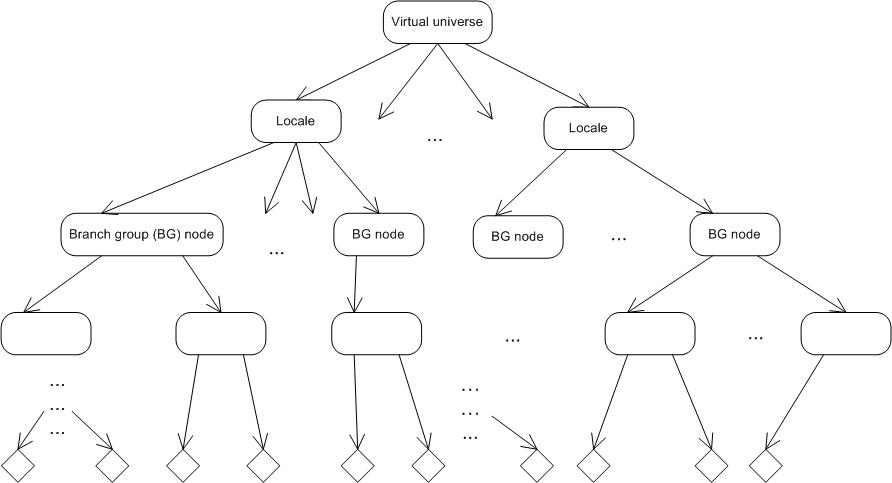
\includegraphics{java3d_diagram_sceny.jpg} 
\caption {Java3D - reprezentacja sceny}
\label {java3d_diagram_sceny}
\end {center}
\end{figure}
 Wśród jego wierzchołków możemy wyróżnić:
\begin{itemize}
\item Group nodes - wierzchołki reprezentujące grupę elementów. Mogą zawierać zero lub więcej dzieci. Grupowanie elementów umożliwia wykonywanie operacji dla całej grupy. Na diagramie \ref{java3d_diagram_sceny} przedstawione są jako zaokrąglone kształty.
\item Leaf nodes - liście reprezentują obiekt tworzący scenę (geometrię, oświtlenie, dźwięk). Nie mogą posiadać dzieci. Na diagramie \ref{java3d_diagram_sceny} występują w postaci rombów.
\end{itemize}
Korzeniem całego grafu jest obiekt klasy \textit{VirtualUniverse} lub dowolnej, dziedziczącej po niej klasie. Graf sceny może posiadać wiele wierzchołków, jednak w większości przypadków jeden jest wystarczający. Obiekt klasy \textit{Locale} jest kontenerem przechowującym kolekcję podgrafów, których korzeniami są instancje klasy \textit {BranchGroup}. Obiekt klasy \textit{BranchGroup} powinien być postrzegany jako jednostka, która po stworzeniu jest kompilowana, a następnie dołączana do grafu reprezentującego wirtualny wszechświat. W dowolnym momencie może zostać odłączana i powtórnie dołączona w inne miejsce.
Tworzenie obiektu 3D przy użyciu Java3D API przebiega następująco:
\begin{enumerate}
\item Tworzony jest obiekt. Ustalane są jego właściwości.
\item Stworzony obiekt dołączany jest do odpowiedniego grafu reprezentowanego przez obiekt BranchGroup.
\item Powstałe grafy w ten sposób grafy są łączone w jedną strukturę reprezentującą wirtualny wszechświat.
\end{enumerate}
Dobrą praktyką jest wspomniane powyżej kompilowanie stworzonych podgrafów przed ich połączeniem. Nie jest ono konieczne ale powoduje  zamianę grafu do wewnętrznego formatu umożliwiającego jego optymalizację. Na uwagę zasługuje fakt, że domyślnie obiekty mogą być modyfikowane jedynie podczas tworzenia podgrafu. Po dołączeniu już stworzonego podgrafu do większej całości informacja o jego obiektach jest oddzielnie zapamiętywana, w sposób przyspieszający operacje dostępu do danych. Można to zmienić wywołując podczas tworzenia obiektu metodę \textit{setCapability} z odpowiednim parametrem.

Przedstawiony powyżej graf sceny jest logiczną reprezentacją renderowanych obiektów.
Do renderingu przygotowanej sceny konieczny jest obiekt klasy Viewer.
Zawiera on wszelkie informacje potrzebne do stworzenia obrazu całej sceny. Z obiektem klasy VirtualUniverse połączony jest
poprzez instancję klasy ViewingPlatform, która inicjalizuje obiekt klasy Viewer dla stworzoneg grafu.
Obiekt klasy Viewer posiada referencje do obiektów klasy View, będących jego lokalnym odpowiednikiem.
Obiekt klasy \text{View} zawiera wszystkie iformacje potrzebne do renderingu pojedynczego elementu sceny oraz referencję do instancji klasy Canvas3D, gdzie opisywany element ma być wyrenderowany.
Jest on połączony z każdym liściem grafu sceny poprzez instancję klasy \textit {ViewPlatform}.
Klasa ViewPlatform odpowiada za inicjalizację obiektu View oraz pozycję, orientację i skalę opisywanego wierzchołka grafu sceny.

\subsubsection{Implementacja modułu wizualizacji}
Moduł wizualizacji zaimplementowany w pakiecie View jest realizacją schematu przedsawionego na diagramie \ref{uml_view}.
\begin{figure}
\begin {center}
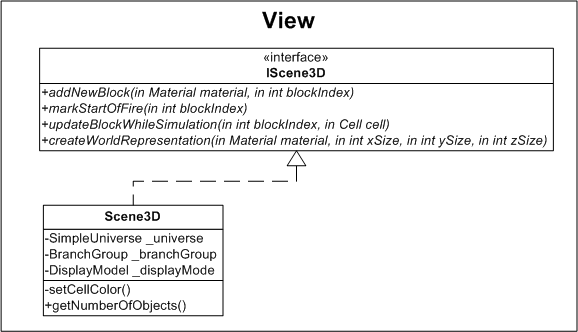
\includegraphics{uml_view.png} 
\caption {Moduł View}
\label {uml_view}
\end {center}
\end{figure}

Klasa Scene3D, implementująca interfejs IScene3D, realizuje przedstawioną powyżej budowę sceny z wykorzystaniem interfejsu Java3D.
Składa się z następujących atrybutów:
\begin{itemize}
\item \_universe - Do budowy korzenia grafu sceny została wykorzystana klasa \textit{SimpleUniverse}. SimpleUniverse pozwala na najprostszą formę inicjalizacji grafu sceny z wykorzystaniem domyślnie tworzonych obiektów klasy \textif{Viewer} oraz \textit{ViewingPlatform}. 
\item \_branchGroup - Obiekt klasy BranchGroup jest podgrafem reprezentującym tworzony budynek. Jest on listą obiektów klasy \textit{TransformGroup}, reprezentujących pojedyncze komórki automatu. Zastosowanie klasy \textit{TransformGroup} umożliwia przemieszczenia poszczególnych
elementów budynku w trakcie działania aplikacji.
\item \_displayMode - DisplyMode odpowiada za tryb wyświetlania wyników symulacji. Może przyjmować jedną z dwóch wartości: TEMPERATURE - powodującą przejście symulacji w tryb wyświetlania rozkładu temperatur podczas pożaru lub REGULAR - przedstawiającą aktualny stan komórki.
\end{itemize}
Interfejs \textot{IScene3D} dostarcza metody umożliwiające wizualizację symulacji. Poniżej przedstawiono ich krótką charakterystykę:
\begin{itemize}
\item \textit{addNewBlock} - dodaje do widoku sceny nowy element knstrukcyjny poprzez zaaplikowanie atrybutów określających wygląd wskazego materiału do określonej przez \textit{blockIndex} komórki. \textif{BlockIndex} jest numerem odpowiadającego elementu z listy \textit{\_branchGroup}. Index jest wyliczany w klasie World, z której wywoływana jest omawiana metoda.
\item \textit{markStartOfFire} - pokazuje źródło pożaru poprzed pokolorowanie odpowiedniej komórki.
\item \textit{updateBlockWhileSimulation} - zmienia wygląd komórki określonej przez \textit{blockIndex} zgodnie z wartościami jej temperatury i materiału oraz uwzględniając aktualny tryb wyświetlania symulacji.
\item \textit{createWorldRepresentation} - tworzy wizualizację automatu komórkowego. Podczątkowy cały automat składa się z komórek wypełnionych tlenem. Metoda \textit{createWorldRepresentation} odpowiada za wypełnienie automatu o wskazanych rozmiarach wytypowanym materiałem (sugerowanym materiałem jest tlen). Tak przygotowany automat możliwy jest do modyfikacji poprzez dodawanie kolejnych elementów konstrukcyjnych lub w wyniku przeprowadzonej symulacji.
\end{itemize}

\subsection {Logika aplikacji}
Logika aplikacji zaimplementowana jest w obrębie pakietu \textit{Model}.
Jego budowę przedstawia diagram \ref{uml_model}.
Główną klasą pakietu \textit{Model} jest \itextit{World}. Zawiera ona strukturę danych reprezentującą autmat komórkowy oraz
zestaw metod umożliwiających przeprowadzanie symulacji.
\subsubsection{World}
Klasa World została zaimplementowana jako \textit{Singleton}, ze względu na fakt
jest unikalności w obrębie aplikacji. 

Strukturą danych, która posłużyła do przechowywania automatu jest trójwymiarowa tablica. Innym kontenerem bardzo często wykorzystywanym do reprezentacji przedstawianego świata w symulacjach jest drzewo ósemkowe, którego użycie również zostało rozważone podczas realizacji projektu Sparkle. Poniżej prezentowane są krótkie rozważania na temat wymienionych struktur wraz z uzasdanieniem wyboru. 

Drzewo ósemkowe to strukturą pozwalająca podzielić trójwymiarowy świat na mniejsze, regularne części. Jest ono tworzone zgodnie z następującymi regułami:
\begin{itemize}
\item Korzeniem drzewa jest sześcian, w którym zawarty jest modelowany świat.
\item Każdy z wierzchołków reprezentuje sześcian będący częścią całego obiektu. 
\item Każdy z wierzchołków nie będący liściem posiada osiem dzieci, reprezentujących sześciany w nim zawarte zgodnie z rysunkiem \ref{drzewo_osemkowe}.
\end{itemize}
\begin{figure}
\begin {center}
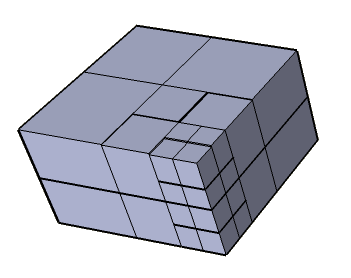
\includegraphics[scale=0.5]{drzewo_osemkowe.png} 
\caption {Podział sceny przy pomocy drzewa ósemkowego}
\label {drzewo_osemkowe}
\end {center}
\end{figure}
Drzewo ósemkowe daje możliwość optymalizacji wykrozystywanej pamięci poprzez przechowywanie jedynie komórek, których stan różni się od stanu rodzica. Komórki identyczne z rodzicem są przez niego reprezentowane, a rodzic taki staje się liściem drzewa. 
Taki sposób przechowania danych jest szczególnie korzystny w przypadku dużej ilości komórek nie biorących udziału w symulacji.
Jest też często wykorzystywany przy renderingu sceny składającej się w znacznej mierze z powietrza, które można zaniedbać.

W przypadku symulacji pożaru, próba adaptacji omawianej struktury okazała się nieefektywna.
Główną przyczyną jest dynamika modelowanego systemu, w którym stan większości komórek zmienia się w krótkim czasie po uruchomieniu symulacji, a kolejne zmiany następują z dużą częstotliwością. Algorytmy propagacji ciepła powodują, że możliwość wyodrębnienia  sześcianu  którego części składowe miałyby stan identyczny z rodzicem należy do rzadkości. Powoduje to, że korzyści płynące ze stosowania wyżej omówionej optymalizacji w przypadku symulacji pożaru są znikome. 
 Bardzo istotnym faktem jest także dodatkowe zużycie pamięci wynikające ze stosowania wskaźnikowej struktury danych. W przypadku gdy drzewo ósemkowe jest drzewem pełnym (każdy z wierzchołków nie będących liściem posiada osiem dzieci) ilość pamięci zużytej przez drzewiastą reprezentajcę przewyższa ilość wykorzystywaną w przypadku implementacji tablicowej.
\begin{figure}
\begin {center}
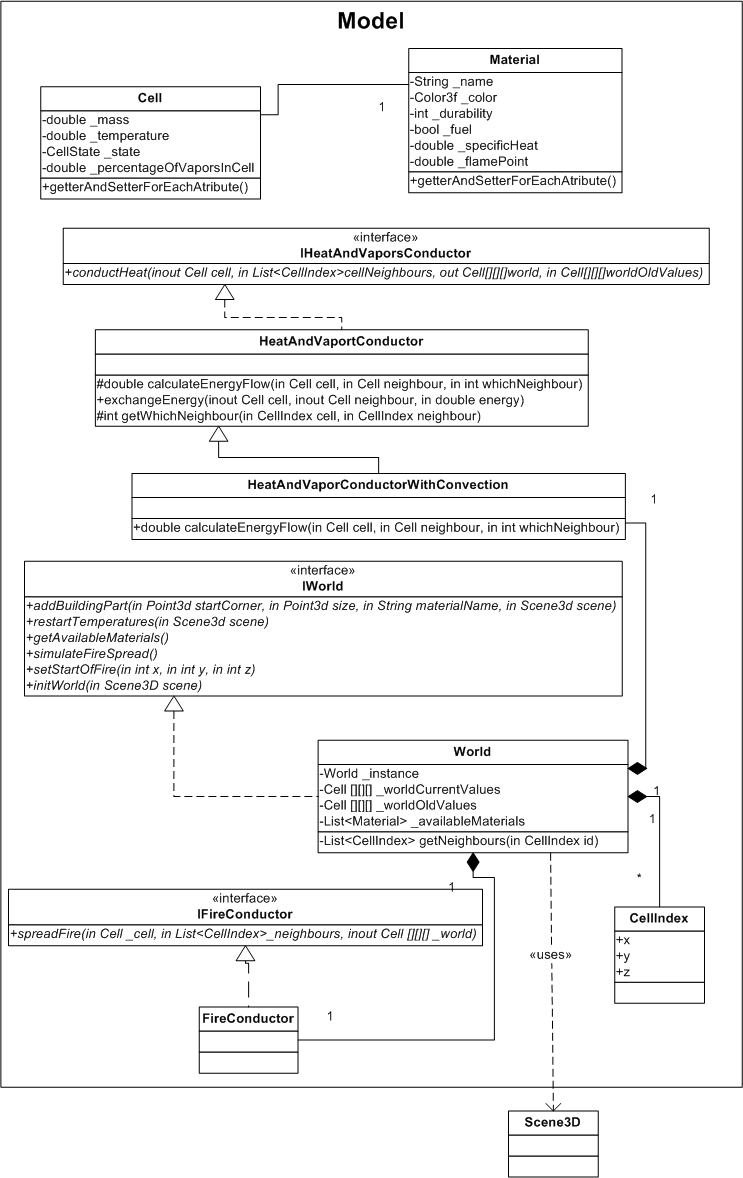
\includegraphics{uml_model.png} 
\caption {Moduł Model}
\label {uml_model}
\end {center}
\end{figure}

Klasa World przechowuje macierz komórek w dwóch egzemplarzach. Podwójne przechowywanie wartości automatu umożliwia odczytywanie parametrów komórki z jednej tablicy, a ich uaktualnianie w drugiej. Taki zabieg nosi nazwę \textit{podwójne buforowanie} czyli \textit{double-buffering} i pozwala uniknąć kierunkowości symulacji. W przypadku nie zastosowania powyższej taktyki temperatura podczas symulacji pożaru rozchodzi się zawsze zgodnie z kierunkiem aktualizacji komórek. Instancja klasy World przechowuje także listę materiałów, które mogą być elementami konstrukcyjnymi budynku. Klasa World zawiera wewnętrzną klasę pomocnicza CellIndex,  która przedstawia index komórki w postaci trzech współrzędnych (x,y,z).

Klasa World impleentuje interfejs IWorld, do którego metod należy:
\begin{itemize}
\item \textit{addBuildingPart} - do odpowiedzialności tej metody należy zmiana materiału komórek wchodzących w skład dodawanego bloku, a także wywołanie odpowiedniej metody klasy Scene3D dokonującej akualizacji widoku podczas edycji budynku. Zadaniem metody addBuildingPart jest zamiana indeksu komórki zapisanego w postaci trójki liczb (x,y,z) na numer odpowiadającej komórki w liście.
\item \textit{restartTemperatures} - metoda wywoływana podczas restartu symulacji. Nadaje wszystkim komórkom parametry domyślne.
\item \textit{getAvailableMaterials} - zwraca listę materiałów, z którym można konstruować budynek.
\item \textit{simulateFireSpread}  - wykonuje jeden przebieg algorytmu aktualizacji automatu komórkowego, wywołując w tym celu metody klas HeatAndVaporConductorWithConvection i FireConducter. Metoda ta jest także odpowiedzialna za wywołanie aktualizacji widoku po każdym przebiegu pętli. Odpowiada za aktualizację macierzy automatu tak aby w każdej chwili macierz, z której czytane są dane była możliwie aktualna z zachowaniem spójności.
\item \textit{setStartOfFire} - ustala punkt startowy pożaru, zmieniając odpowiednio wartości wskazanej komórki.
\item \textit{initWorld} - inicjalizuje autmat wartościami domyślnymi. Domyślnym materiałem wypełniającym przestrzeń jest Tlen. Temperatura komórek na początku działania aplikacji ustawiana jest na $20^\circ C$. Metoda ta odpowiada także, za wywołanie funkcji tworzącej graficzną reprezentację modelu (\textit{createdWorldRepresentation} z klasy \textit{Scene3D}).
\end{itemize}
Ponadto klasa World zawiera metody pomocnicze, do których należy:
\begin{itemize}
\item \textit{getNeighbours} - zwracająca listę indeksów sąsiadów badanej komórki
\item \textit{updateOldValues} - aktualizująca macierz wartości do odczytu
\end{itemize}

\subsubsection{Cell i Material}
To klasy, które zgodnie z opisem zawartym w rozdziale \ref{cha:projekt} zawierają zestaw prywatnych atrybutów określających  odpowiednio stan komórki i właściwości materiału. Z każdym atrybutem związane są metody get i set, kontrolujące dostęp do zmiennych. 

\subsubsection{FireConductor}
Klasa FireConductor odpowiada za rozprzestrzenianie ognia zgodnie z algorytmem opiany w rozdziale \ref{cha:Algorytm}.
Implementuje interfejs IFireConductor zawierający metodę \textit{spreadFire}. Metoda ta jest odpowiedzialna za zmianę stanu komórki
z naturalnego na palący i odwrotnie.

\subsubsection{HeatAndVaporsConductor oraz HeatAndVaporConductorWithConvection}
Do bardziej rozbudowanych klas należy HeatAndVaporsConductor oraz HeatAndVaporConductorWithConvection.
Klasa HeatAndVaporsConductor implementuje interfejs IHeatAndVaporsConductor, definiując metodę \textit{conductHeat}.
Metoda ta wywoływana jest dla każdej komórki automatu, w każdym obiegu algorytmu.
Odpowiada za obliczenie energii przepływającej między badaną komórką i jej wszystkimi sąsiadami oraz symulację wymiany ciepła, 
której wynikiem jest uaktualnienie temperatur komórek. Wszystkie obliczenia przeprowadzane są zgodnie z metodami odpisanymi w rozdziale \textit{Algorytm}. W ich realizacji wykorzystywane są pomocnicze metody: 
\begin{itemize}
\item \textit{calculateEnergyFlow} - odpowiadająca za obliczenie ilości energii przepływającej między dwoma komórkami \\ 
oraz 
\item \textit{exchangeEnergy} - symulująca wymianę ciepła. 
\end{itemize}
Klasa HeatAndVaporsConductor podczas wyliczania przepływającej energii uwzględnia jedynie zjawisko przewodnictwa cieplnego, zaniedbując konwekcję. 

Symulacja konwekcji, jak wyjaśniono w rozdziale \ref{cha:Algorytm} opiera się na ułatwieniu przepływu ciepła do górnych sąsiadów komórki. Konwekcja jest więc szczególnym przypadkiem przewodnictwa, występującym w powietrzu. Zgodnie z powyższym, klasą realizującą konwekcję jest HeatAndVaporConductorWithConvection dziedzicząca po klasie HeatAndVaporsConductor. Przedefiniowana w  klasie potomnej metoda \textit{calculateEnergyFlow} wywołuje odpowiadającą funkcję klasy nadrzędnej, a następnie wprowadza do wyliczonej zgodnie z regułami przewodnictwa energii zmiany wywołane konwekcją. Zmiany te aplikowane są tylko w przypadku gdy badana komórka oraz komórka sąsiednia, z którą następuje wymiana ciepła są powietrzem. Metoda \textit{exchangeEnergy} poza wymianą ciepła między sąsiadującymi komórkami implementuje także przekazywanie drogą konwekcji oparów koniecznych do zapłonu komórki.

\subsection {Moduł obsługi zdarzeń}
Głównym zadaniem modułu obsługi zdarzeń jest obsługa interakcji z użytkownikiem. Implementacja modułu zawarta jest w pakiecie \textit{Controller}.